\documentclass[10pt]{amsart}
\usepackage{amssymb,amsthm,amsmath,graphicx,booktabs,microtype,float}
\usepackage[letterpaper,left=2.25cm,right=2.25cm,top=2.2cm,bottom=2.2cm]{geometry}
\usepackage[hidelinks]{hyperref}
\newtheorem{defn}{Definition}[section]
\title[Residual spectral graph learning]{Residual Spectral Graph Learning for Connectivity-Loss Estimation under Multi-Edge Disruptions}
\author{Le Van Truong}
\address{University of Science, Vietnam National University Ho Chi Minh City}
\date{September 2026}
\begin{document}
\begin{abstract}
We estimate algebraic-connectivity loss after simultaneous road-network edge
disruptions. The proposed model learns a bounded graph-neural correction to an
interpretable first-order Fiedler approximation. We compare eight learned
configurations and the analytical baseline under independent and spatially
clustered failures, using graph-disjoint synthetic splits and zero-shot transfer
to five OpenStreetMap (OSM) networks. Results are replicated with five seeds and
uncertainty is computed by resampling seeds, not individual scenarios. On OSM,
the residual model obtains mean absolute error (MAE) 0.097 (95\% seed-bootstrap
CI 0.091--0.102) for independent failures and 0.090 (0.071--0.124) for spatial
failures. Relative to a direct GCN, paired MAE improvements are 0.0085
(0.0039--0.0131) and 0.0121 (0.0026--0.0247), respectively. Fiedler-node and
coordinate ablations are inconclusive, indicating that the explicit residual
prior provides the robust gain. Exact OSM eigendecomposition averages 5.09 ms
per scenario; the first-order update requires 0.018 ms and learned inference
0.44--0.67 ms on a CPU. This is structural disruption analysis, not hazard or
traffic-flow prediction.
\end{abstract}
\maketitle

\section{Introduction}
Removing a few links can change global road-network connectivity. Exact
spectral recomputation is reliable but may be expensive in large scenario
studies, while a local sensitivity is fast but ignores finite interactions.
Graph neural networks (GNNs) can represent such interactions, yet direct
end-to-end learning may discard useful mathematics. We therefore ask whether a
GNN should predict connectivity loss directly or correct a spectral prior.

Our contributions are: (i) a residual spectral--GCN for multi-edge disruption;
(ii) separation of an explicit spectral prior from Fiedler node features;
(iii) independent and spatial-cluster failures on five OSM networks; (iv)
direct GCN, Deep Sets, summary-MLP, feature, and residual ablations; and (v)
seed-level paired uncertainty, runtime, and regime-specific error analysis.

\section{Related work and novelty positioning}
Fiedler's algebraic connectivity $\lambda_2$ characterizes connectedness and
underlies spectral robustness analysis~\cite{fiedler1973,jamakovic2008}.
Its eigenvector gives an edge-weight derivative, but summing derivatives is a
local approximation and need not capture simultaneous finite deletions.

Road robustness has been studied under random, targeted, and localized link
failures. Synthetic road graphs permit controlled topology experiments
~\cite{sohouenou2020}; hazard-independent multi-link analysis also demonstrates
that conclusions depend on disruption multiplicity~\cite{sohouenou2021}. Our
target is structural connectivity, complementary to travel time, flow, or
accessibility and not a substitute for them.

GCNs propagate local information over graph adjacency~\cite{kipf2017}, whereas
Deep Sets supplies a permutation-invariant baseline without message passing
~\cite{zaheer2017}. Physics-informed graph learning combines analytical
structure and learned components~\cite{sanchezgonzalez2018}. We do not claim
the first use of GNNs or spectral robustness. The novelty is the controlled,
leakage-resistant comparison of node-level spectral information versus an
explicit residual prior, across two failure processes and five unseen OSM
networks, with paired seed-level inference and computational profiling.

\section{Formulation and models}
Let $G=(V,E,w)$ be connected and undirected, $L=D-A$ its combinatorial
Laplacian, and $0=\lambda_1\leq\lambda_2\leq\cdots$ its eigenvalues.
\begin{defn}[Relative connectivity loss]
For disrupted edges $S\subseteq E$,
\begin{equation}
y(G,S)=\operatorname{clip}\left(1-\lambda_2(G-S)/\lambda_2(G),0,1\right).
\label{eq:target}
\end{equation}
Disconnection therefore gives $y=1$.
\end{defn}
If $u_2$ is a unit Fiedler vector and $\lambda_2$ is simple, then
$\partial\lambda_2/\partial w_{ij}=(u_{2,i}-u_{2,j})^2$. Our analytical
baseline is
\begin{equation}
\widehat y_{\rm spec}=\operatorname{clip}\left(
\frac{\sum_{(i,j)\in S}w_{ij}(u_{2,i}-u_{2,j})^2}{\lambda_2(G)},0,1\right).
\label{eq:spectral}
\end{equation}

The ScenarioGCN receives the damaged adjacency and node features comprising
normalized original degree, disrupted-edge incidence, absolute normalized
Fiedler coordinate, and two normalized spatial coordinates. Three 48-unit GCN
layers are followed by mean--max pooling and a two-layer head. The residual
variant predicts
\begin{equation}
\widehat y_{\rm res}=\operatorname{clip}
(\widehat y_{\rm spec}+\tanh r_\theta(G,S),0,1).
\end{equation}
We compare direct and residual versions with all features, without Fiedler, and
without coordinates. Additional baselines are a Deep Sets node encoder and an
MLP using graph summary statistics. All learned models use the same split,
AdamW, mean-squared error, at most 80 epochs, and validation early stopping.

\section{Experimental design}
\subsection{Synthetic data and failure processes}
Connected random geometric graphs contain 35--65 nodes with inverse-length
edge conductance. Each seed has 1,600 balanced scenarios (800 per failure
mode): 1,120 train, 240 validation, and 240 test examples, split by base-graph
identifier. No damaged version of a training graph can enter validation or
test. Independent failure samples 1--8 edges uniformly. Spatial failure
chooses a random epicentre and removes the requested number of edges whose
midpoints are nearest to it.

\subsection{Five-network OSM transfer}
OSMnx~\cite{boeing2017} downloaded 650-m drivable networks around five
Vietnamese sites. Directed multigraphs were simplified, converted to undirected
simple graphs, and restricted to their largest connected component. Conductance
is $100/\text{length}_{\rm m}$. Table~\ref{tab:osm} spans different sizes and
densities. For every seed, site, and failure process, 100 scenarios were
generated, giving 1,000 OSM scenarios per seed. OSM data are never used for
training, early stopping, or model choice.

\begin{table}[H]
\centering
\caption{Cached OSM networks. Density is $2|E|/(|V|(|V|-1))$.}
\label{tab:osm}
\begin{tabular}{lrrr}
\toprule Site & Nodes & Edges & Density\\ \midrule
HCMUS (Ho Chi Minh City)&163&221&0.0167\\
VIASM (Hanoi)&206&301&0.0143\\
Da Nang&142&203&0.0203\\
Can Tho&114&178&0.0276\\
Da Lat&48&55&0.0488\\ \bottomrule
\end{tabular}
\end{table}

\subsection{Statistics and runtime}
Metrics are calculated within each seed. Reported 95\% intervals resample the
five seed-level values 10,000 times. Comparisons use within-seed paired
differences; scenarios sharing a graph or seed are never treated as independent
replicates. Runtime uses one PyTorch CPU thread on the same 16-logical-CPU
Windows machine, and includes per-scenario prediction but excludes training and
data loading.

\section{Results}
\begin{table}[H]
\centering
\caption{OSM zero-shot results: seed mean MAE [95\% seed-bootstrap CI] and
Spearman correlation.}
\label{tab:main}
\small
\begin{tabular}{lcc|cc}
\toprule &\multicolumn{2}{c|}{Independent}&\multicolumn{2}{c}{Spatial cluster}\\
Method&MAE&$\rho$&MAE&$\rho$\\ \midrule
Spectral first order&0.502 [0.482,0.521]&0.391&0.650 [0.643,0.657]&0.324\\
Summary MLP&0.281 [0.240,0.320]&0.819&0.347 [0.269,0.425]&0.787\\
Deep Sets&0.114 [0.105,0.123]&0.765&0.143 [0.122,0.164]&0.789\\
Direct GCN&0.106 [0.100,0.112]&0.848&0.102 [0.077,0.148]&0.841\\
Residual GCN&\textbf{0.097 [0.091,0.102]}&\textbf{0.903}&0.090 [0.071,0.124]&\textbf{0.896}\\
Residual, no Fiedler&0.096 [0.090,0.101]&0.901&\textbf{0.078 [0.067,0.090]}&0.889\\
Residual, no coordinates&0.098 [0.092,0.102]&0.901&0.095 [0.073,0.122]&0.895\\
\bottomrule
\end{tabular}
\end{table}

Residual-full improves upon direct-full by paired MAE 0.0085
[0.0039,0.0131] for independent and 0.0121 [0.0026,0.0247] for spatial
failures. On synthetic graphs the improvements are 0.0253
[0.0106,0.0400] and 0.0160 [0.0048,0.0241]. Thus the residual formulation is
the stable contribution. In contrast, every paired MAE CI comparing
residual-full with its no-Fiedler or no-coordinate variant contains zero. The
spatial OSM point estimate even favours no-Fiedler. These features should be
regarded as optional under the present power, not established necessities.

\begin{figure}[H]
\centering
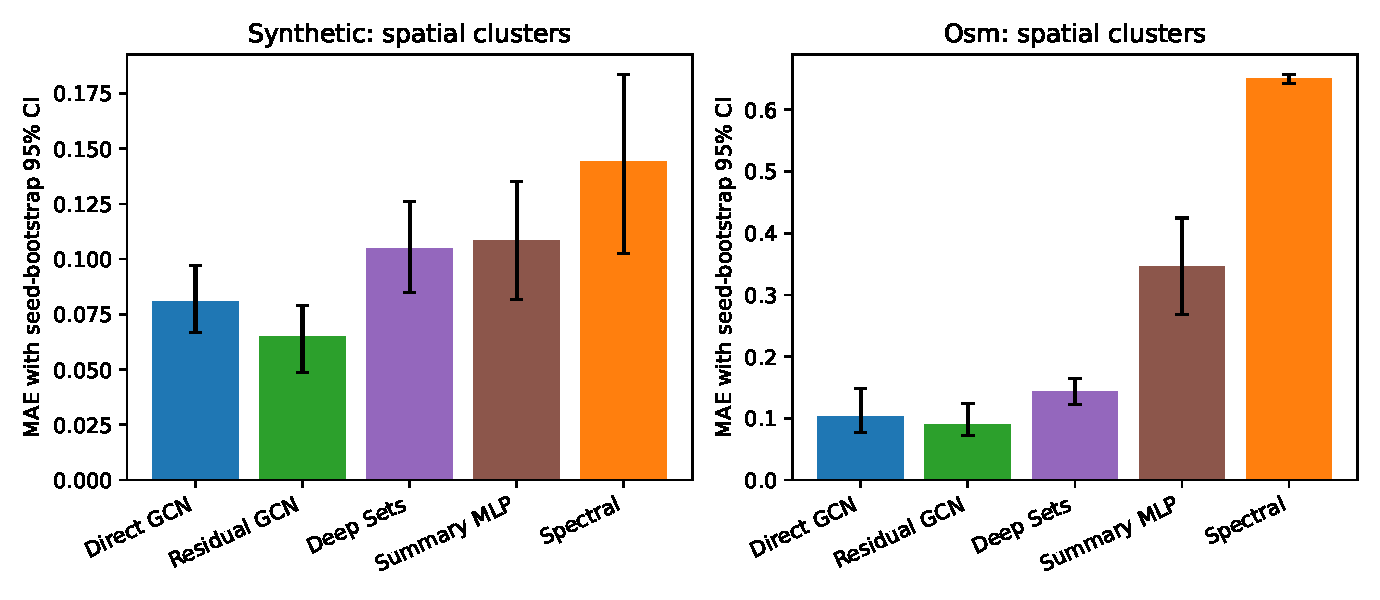
\includegraphics[width=.88\textwidth]{../outputs/paper_summary/paper_primary_results.pdf}
\caption{Spatial-cluster performance in the synthetic and OSM domains. Error
bars are 95\% intervals from seed-level bootstrap.}
\label{fig:main}
\end{figure}

\subsection{Runtime}
\begin{table}[H]
\centering
\caption{Mean per-scenario runtime on OSM (milliseconds).}
\label{tab:runtime}
\begin{tabular}{lr@{\qquad}lr}
\toprule Method&ms&Method&ms\\ \midrule
Exact eigendecomposition&5.094&Spectral first order&0.018\\
Summary MLP&0.442&Deep Sets&0.430\\
Direct GCN&0.502&Residual GCN&0.674\\
\bottomrule
\end{tabular}
\end{table}
The analytical approximation is about 287 times faster than exact recomputation;
residual inference is about 7.6 times faster. These ratios are implementation-
and graph-size-specific. Mean training time ranges from 60 s (summary MLP) to
150 s (slowest GCN ablation), and residual-full averages 121 s per seed on CPU.

\subsection{Error regimes}
For residual-full on pooled OSM failure modes, seed-mean MAE is 0.070 for
connected damaged graphs and 0.112 after disconnection. By failed-edge count it
is 0.090 (one), 0.116 (two--three), 0.089 (four--five), and 0.081 (six or more),
so error is not monotone in disruption count. Site MAE is 0.041 Can Tho, 0.061
VIASM, 0.088 Da Nang, 0.089 HCMUS, and 0.189 Da Lat. The dense but much smaller
Da Lat graph is hardest, warning against attributing error to density alone.
No evaluated scenario clipped Equation~\eqref{eq:spectral} at one; consequently
the requested clipped-versus-unclipped comparison is undefined rather than
silently omitted. The poor spectral OSM MAE instead reflects large
non-saturating overestimates.

\section{Discussion and limitations}
The explicit prior substantially improves a direct GCN even when the prior
alone transfers poorly. It supplies useful rank structure, while the learned
correction calibrates nonlinear finite-deletion effects. Deep Sets is
competitive only in selected regimes and the summary MLP loses substantial
accuracy, supporting the use of graph structure.

Five seeds permit uncertainty reporting but not high-powered claims about small
feature effects. The OSM samples cover only 650-m neighbourhoods in Vietnam;
Da Lat also differs in size as well as density. Spatial clusters are geometric
proxies, not measured floods, landslides, or construction events. Algebraic
connectivity ignores traffic demand, direction, capacity, travel time, and
recovery. Future work should use larger networks, blocked geographic transfer,
licensed hazard layers, and sparse/iterative eigensolvers.

\section{Conclusion}
Across both disruption processes and both domains, learning a correction to a
Fiedler approximation is more reliable than direct GCN regression. Full
feature ablation does not support strong claims for Fiedler node coordinates or
spatial coordinates individually. Multi-area transfer, seed-paired statistics,
runtime profiling, and explicit failure-regime analysis make the result suitable
as a reproducible poster study while delimiting its real-world interpretation.

\section*{Reproducibility statement}
The repository includes cached GraphML, all generators and models, raw-output
schemas, a 10,000-resample analysis script, and \texttt{reproduce\_all.ps1}.
Seeds are 11, 22, 33, 44, 55. The recorded environment is Python 3.13.11;
NumPy 2.4.4; SciPy 1.17.1; NetworkX 3.6.1; pandas 2.2.3; scikit-learn 1.9.0;
PyTorch 2.11.0 (CPU); Matplotlib 3.11.1; OSMnx 2.1.1; and GeoPandas 1.1.4.
Hardware is an AMD64 Family 25 Model 68 system with 16 logical CPUs; CUDA was
unavailable and no GPU was used. OSM data are copyright OpenStreetMap
contributors under the ODbL~\cite{osm}.

\begin{thebibliography}{10}
\bibitem{fiedler1973} M. Fiedler, \emph{Algebraic connectivity of graphs},
Czechoslovak Math. J. 23 (1973), 298--305.
\bibitem{jamakovic2008} A. Jamakovic and P. Van Mieghem, \emph{On the
robustness of complex networks by using the algebraic connectivity}, Networking
2008, LNCS 4982, 183--194.
\bibitem{sohouenou2020} P.Y.R. Sohouenou, P. Christidis, A. Christodoulou,
L.A.C. Neves, and D. Lo Presti, \emph{Using a random road graph model to
understand road networks robustness to link failures}, Int. J. Crit. Infrastruct.
Prot. 29 (2020), 100353.
\bibitem{sohouenou2021} P.Y.R. Sohouenou, L.A.C. Neves, A. Christodoulou,
P. Christidis, and D. Lo Presti, \emph{Using a hazard-independent approach to
understand road-network robustness to multiple disruption scenarios}, Transp.
Res. Part D 93 (2021), 102672.
\bibitem{kipf2017} T.N. Kipf and M. Welling, \emph{Semi-supervised
classification with graph convolutional networks}, ICLR, 2017.
\bibitem{zaheer2017} M. Zaheer et al., \emph{Deep Sets}, NeurIPS 30, 2017.
\bibitem{sanchezgonzalez2018} A. Sanchez-Gonzalez, N. Heess, J.T. Springenberg,
J. Merel, M. Riedmiller, R. Hadsell, and P. Battaglia, \emph{Graph networks as
learnable physics engines for inference and control}, ICML, 2018.
\bibitem{boeing2017} G. Boeing, \emph{OSMnx: New methods for acquiring,
constructing, analyzing, and visualizing complex street networks}, Comput.
Environ. Urban Syst. 65 (2017), 126--139.
\bibitem{osm} OpenStreetMap contributors, \emph{OpenStreetMap}, 2026,
\url{https://www.openstreetmap.org/copyright}.
\end{thebibliography}
\end{document}
